\section{Zielsetzung}
Ziel dieses Versuchs ist die Untersuchung von Dispersion am Glasprisma.
Dazu zählt die Bestimmung  der Dispersionskurve.
\section{Theorie}
tritt eine Lichtwelle in Materie ein kommt es zu Wechselwirkungen zwischen der Welle und den Elektronen.
Da die Ausbreitungsgeschwindigkeit v in Licht geringer ist als die Geschwindigkeit c im Vakuum kommt es
beim übertreten in eine andere Schicht zu einer Richtungsänderung.
Diese wird als Brechung bezeichnet.
Der Brechungsindex n kann beschriben weren durch
\begin{equation}
  n := \frac{c}{v} = \frac{v_1}{v_2}
\end{equation}
Die Ausbreitungsgeschwindigkeit von Licht in Materie ist eine frequenzabhängige Größe.
Somit ist der Brechungsindex eine Funktion der Frequenz \omega oder der Wellenlänge \lambda.
\begin{equation*}
  n =f(\lambda)
\end{equation*}
Diese Funktion ist  die sogennate Dispersionskurve.
Mit ihr ist es möglich die chromatische Aberration zu kompensieren.\\
Tritt ein Lichtstrah im Winkel $\alpha$ auf eine Grenzfläche zwischen zwei unterschiedlichen Materiaien,
ändert dieser seine Richtung und breitet sich mit dem Winkel $\beta$ aus.
Der Zusammenhang zwischen Winkel und Geschwindigkeit ergibt sich durch das Huygenssche Prinzip.
Dieses besagt, dass jeder Punkt einer Welle ein Ausgangspunkt einer neuen Elementarwelle ist.\\
Aus diesem kann das Snelliussche Brechungsgesetz hergeleitet werden.
Es beschreibt die Richtungsänderung eines Lichtstrahls durch
\begin{equation}
  n = \frac{\sin\alpha}{\sin\beta} = \frac{v_1}{v_2}
\end{equation}
\newline
Mit Hilfe der maxwellschen Theorie der elektromagnetischen Wellen, kann die Dispersionsgleichung hergeleitet werden.
Um die Dispersion vom sichtbaren Spektralbereich in Gläsern zu beschreiben, eignen sich zwei Formel
\begin{align}
  n^2(\lambda) &= A_0 + \frac{A_2}{\lambda^2}+\frac{A_4}{\lambda^4}+...\\
  \label{eqn:n1}
  n^2(\lambda) &= 1- A'_2\lambda^2 - A'_4\lambda^4-...
  \label{eqn:n2}
\end{align}
Die durch (3) und (\ref{eqn:n2}) beschriebenen Kurven sind in Abbildung \ref{fig:n} zu sehen.

\begin{figure}[H]
\centering
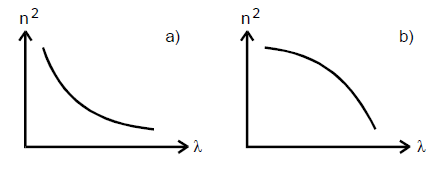
\includegraphics[width=\textwidth]{n.png}
\caption{Gestalt der Dispersionskurve a) nach (3) und b) nach (\ref{eqn:n2})}\cite{anleitung}
\label{fig:n}
\end{figure}

Dabei gilt für (3) für alle $\lambda$
\begin{equation*}
  \frac{d^2n^2(\lambda)}{d\lambda^2}>0
\end{equation*}
und für (\ref{eqn:n2})
\begin{equation*}
  \frac{d^2n^2(\lambda)}{d\lambda^2}<0
\end{equation*}

Die Abnahme des Brechungsindex mit zunehmender Wellenlänge wird dabei als normale Dispersion bezeichnet.
Anormale Dispersion ist die Bezeichnung für die zunahme des Brechungsindex bei zunehmender Wellenlänge.


\section{Durchführung}
Zunächst wird die Quecksilber-CD-Lampe eingeschaltet.
Das Glasprisma wird wie in Abbildung \ref{fig:6} zu sehen auf die Apparatur gesetzt.
Die Lampe wird so eingestellt, dass die einzelnen Spektrallinien scharf zu erkennen sind.
%scheibe auf 0° drehen.
\begin{figure}[H]
\centering
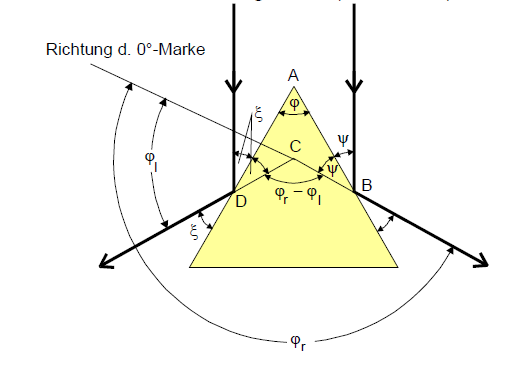
\includegraphics[width=\textwidth]{6.png}
\caption{Bestimmung des Winkels $\varphi$ zwischen den brechenden Oberflächen}\cite{anleitung}
\label{fig:6}
\end{figure}
Es ist eine weiße Linie zu erkennenen.
Diese wird auf das Fadenkreuz gelegt.
Die Messung wird sieben mal durchgeführt.
Der Winkel kann mit
\begin{equation}
  \varphi = \frac{1}{2}(\varphi_r-\varphi_l)
  \label{eqn:phi}
\end{equation}
berechnet werden.

Im nächsten Teil des Versuchs wir das Prisma wie in Abbildung \ref{fig:4} aufgestellt.
Die weiße Linie wird auf die einzelnen Spektrallinien gelegt und der Winkel wird gemessen.
Danach wird das Prisma wie in Abbildung \ref{fig:5} gedreht und die Messung wiederholt.

\begin{figure}[H]
\centering
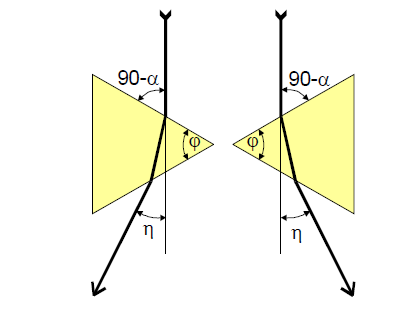
\includegraphics[width=\textwidth]{4.png}
\caption{Bestimmung des Brechungswinkels $\eta$}\cite{anleitung}
\label{fig:4}
\end{figure}

\begin{figure}[H]
\centering
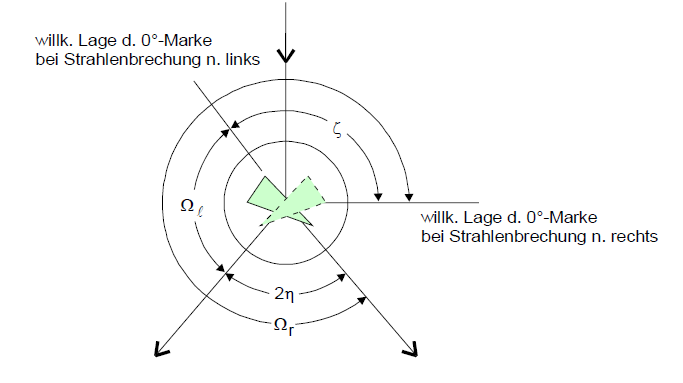
\includegraphics[width=\textwidth]{5.png}
\caption{Darstellung der Messgrößen $\Omega_l$ und $\Omega_r$}\cite{anleitung}
\label{fig:5}
\end{figure}
$\eta$ kann mit Formel
\begin{equation}
  \eta = 180 - (\Omega_r-\Omega_l)
\end{equation}
bestimmt werden.
